%!TEX root = project.tex






\begin{document}

\hfill \break     
\large
\hfill \break 
\textbf{Abstract} \hfill \break 

\textbf{Student-Mania -} 
Communication is the key right now. With the state of the world and what’s happening right now it is more important than ever for students that are working on their education to be able to communicate with one another. Taken this into account we decided to create a website where all the students would be able to share notes and be able to communicate and ask questions to do with their workloads. When deciding on our project we were told to try and solve a problem, as students this hit close to home for the three of us.   
When students are working from home a lot of different websites are needed \textit{( Discord\cite{ref6},Teams\cite{ref7} and LearnOnline\cite{ref8})} are just to name a few. It can be difficult for non-computer students to keep track of all these applications. Trying to solve this problem for students and trying to help them organize it into one website that could cover all of a student’s needs without them having to navigate and deal with too many applications.  Our application will let the user login, ask questions, and have access to chat boxes and chat rooms for students to meet and discuss course work in real time.   


\hfill \break 

Keywords:

\begin{itemize}
  \item Online learning
  \item peer to peer communication
  \item cloud based hosting
  \item file sharing
  \item Student resources
\end{itemize}

\chapter{Introduction}
\section{Communication tools}

Given the task to join as a group and come up with a project between us, after meeting with our supervisor Mark Campbell we decided to set up a team’s meeting every week to discuss/plan and work on or project for the coming months.
Before any plans or ideas were decided on, we created a mind map for what our project would be, for the goals we wanted to reach and for each other’s parts within the project. We set up meetings with our supervisor and weekly meetings for the group, where  we would work on the project together so we would all understand what we were creating.


\section{Github repository}

Next up was the creation of a Github repository where we would all be contributors to the project and work on it individually as needed. We also added mark to this repository as our supervisor. \hfill \break  
\hfill \break
GitHub Repository for the project:

\url{https://github.com/GallagherStephen/4thYearProject-Dissertation}

\hfill \break
Screencast for the project:

\url{https://youtu.be/wLuYDjyjU3g}

\hfill \break
\begin{figure}
    \centering
    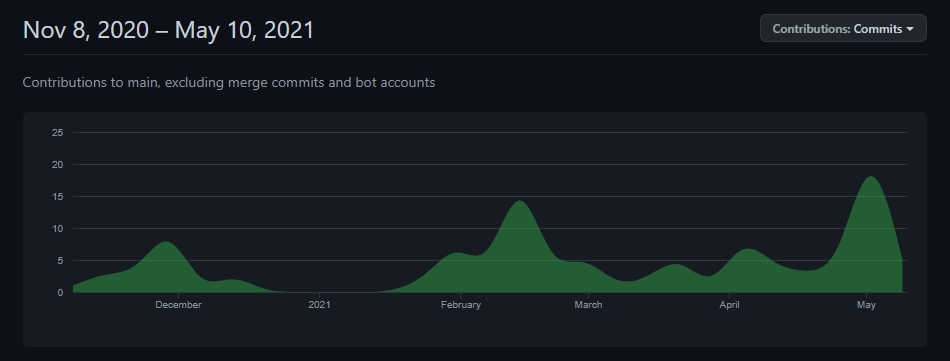
\includegraphics[width=.6\textwidth, inner]{images/graph.png}
    \caption{ }
    \label{fig:my_label}
\end{figure}

\hfill \break
The main factors we decided on for our project, were “what would be some way to help” and “what do students need”. With this in mind we decided to choose a project that would be a benefit to students as we are currently students ourselves and figured it could be an issue that affects students and their way of learning or living as a student.
One of the most important aspects of this project was working as part of a team with other peers.\hfill \break
\hfill \break
To assist us with this project and collaborate, we used Github\cite{ref5} to save and archive our project on a repository that we could all view and then use to share our work with one another. Github is a service that hosts software development and allows you to manage the various versions of your code. Users may either share their repositories with others or make them private to restrict access. This makes collaborating as part of a team much easier and helps the team to monitor who is doing what and when. Another advantage that Github provides is the ability for the user to rollback their code if any bugs or failures were submitted to their repository. Users should use branches to avoid corrupting the master branch of code, allowing for seamless collaboration between teammates.

\section{Ideas}
Some of the ideas were a “delivery services” for food or other items and a “Lift Sharing” for students that don’t live near the college and need to travel by public transport which may not be available to the student. 
Car and rugby apps were some other ideas we had but decided as a group to build a student learning application that focuses on communication , problem solving and ease of use for students with their classmates. 

\section{Motivation of project}
A \textit{Discord/Teams/LearnOnline} type of website/application would be a great benefit to students by helping them keep track of classes and sharing of notes. This application would be designed to be a one stop shop for all student’s needs online, connecting them with their classmates. Communication and friendly interface will be the key to this website/application being useful and successful.\hfill \break

A questionnaire is something worth considering for this project because it will provide us with valuable input about what other students across different courses are thinking, while allowing their voices to be heard in the application's design. This application will cater to a wide range of students not only linked with computer courses.
As a group, completing this project we will all have to work together as much as possible and communicate on the work that is being conducted. With the situation the world is currently in, video calls will play a big factor with regards to communication.\hfill \break

Another form of software we have decided to use was Trello\cite{ref9}, which is an online managing and note tracking website that we as a group can use to track our progress, while designing and building our project. This will let us all monitor and keep track of our work online as a group while being able to add tasks or move them to the completed sections. 
It was our supervisor Mark Campbell that suggested to use Trello as there will be a heavy workload ahead in the coming weeks that will be difficult to keep track of each tasks in real time. Trello is the same as a white board where teammates can leave lists or tasks like sticky notes and removed them when we achieved goals we set weekly. Trello has been a huge support in completing our weekly steps and staying on track with the project.\hfill \break


\section{Project goal}


For our group, we wanted to tackle a problem, so after some deliberation and brainstorming, we decided on a communications website that would allow students to talk and collaborate when needed while working on projects or assignments. For us as a group, communication was the number one goal we set for ourselves while designing and creating this project. This will allow us to assist fellow students through these difficult times. At the time of planning our project, we had great intentions for our early prototype of the project with the goals and objectives we set for ourselves.

If we continue with development on this project in future, one of the main features we would like to add in is one-to-many video calls, which would enable more people to engage in video calls at the same time. Another functionality would be the ability to login using social networking accounts such as \textit{Facebook\cite{ref10}, Twitter\cite{ref11}, and Instagram\cite{ref12}}. 


\chapter{Literature Review on Communication Platforms}
\section{Goals}
The goal of this platform was to make communication easier for students. According to our research findings, students tend to use multiple platforms to cover their workload from classes and lectures. When we were building our platform, we wanted to help students eliminate the need to use multiple platforms and reduce that need to a single platform that could meet all of a student's needs.
Our main finding from our research was that students required multiple platforms to complete their daily workloads. If a student could complete all of these tasks on a single platform, it would be easier, less stressful, and save time overall.

\section{Introduction}

Adapting to new online learning methods is one of the most significant changes for students during this pandemic. In this day and age, communication is the most important factor in education. Online learning and communication between students and lecturers are at the forefront of planning and discussion, thanks to platforms such as \textit{Microsoft Teams, LearnOnline, and Discord}, to name a few.
Even in these difficult times, students must be able to continue their studies. People can stay in touch and continue their education thanks to technologies that connect to the internet. Students are currently communicating with one another through the platforms mentioned above.
In this literary review, we will look at creating our own communications platform for students as well as discussing other platforms from which we drew inspiration to create our own specialized platform. We will discuss the platforms that students are currently using to learn online, along with the benefits and drawbacks of using these applications, as well as what students need from these platforms and how they help students.


\section{Secondary research}
Online Learning 

Prior to the pandemic, online learning was used whenever a student was unable to attend a class or lecture for any number of reasons; however, it was only since the pandemic outbreak that online learning has taken on a more prominent role within the education system. One of the main disadvantages of online learning is the requirement for a stable internet connection and the devices that allow students to work remotely.
The \textit{Discord} platform was created to allow 'gamers' to stream their games to their fans and communicate with them directly via video, voice, and text boxes. Users can set up their own servers for their own use and invite people to join their servers in order to build a fan base on private channels. This allows the streamer with the help of moderators to control the server and supervise who joins, which can cut out some of the toxic content and attitude some users may display.

Microsoft Teams is designed for use by lecturers to share content with their students and businesses for day to day work. Microsoft Teams is a popular workplace application for video conferencing, chat boxes, and file storage. Teams has some great features that Discord does not have, such as a calendar that tracks meetings and classes. Teams also has a feature that allows control to be passed to another user from their computer remotely. This is a great feature when a student is stuck on a subject, the student can allow their lecture to control their computer to solve their issue.  \cite{ref1} \hfill \break



When compared to students who were given the same quiz after an in-class lecture, education taught online using a gaming style teaching practice, such as “Kahoots,”\cite{ref13} showed a higher percentage of students participated and successfully completed the quiz. This demonstrates how difficult it can be to keep a student focused on their work and projects during lectures. Moving all lectures, labs, and classes to an online platform can be challenging, not to mention the hardware required to get students and lecturers set up to handle online teaching. When compared to students who completed in-class one-time quizzes, these gamification scenarios produced very high results. This may be due to the format of the questions used in the online quizzes, multiple choice and true or false, but students reported that using this format was easier to learn. \cite{ref2} \hfill \break



This article discusses how well Discord could be used in an online learning environment, how students feel about its use, and whether Discord could be used more practically with its features.
The interface, interactivity, feedback, and interaction sections in Discord were some of the most popular features among students. Students expressed dissatisfaction with the unstable internet connection and the device capability, which could be on the low side at times. According to the findings of this study, the benefits of using Discord outweigh the drawbacks of using this platform. \cite{ref3} \hfill \break



When it comes to online learning and using the platform to communicate with fellow students and keep in touch with lecturers, most students have found Microsoft teams to be extremely helpful. Teams also has some fantastic features, such as a calendar, chat and share files. Emails that will be used to schedule Team meetings can be used to update the calendar. Students can use this to organize their workload and manage their time on projects and assignments. \cite{ref4} \hfill \break



There are numerous terms that can be used to describe online learning, and one of them is virtual education. When the pandemic hit, lectures and classes went virtual. Virtual environments are intended to bring people together and allow them to interact virtually with their peers as well as their teachers/lecturers. E-learning does not appear to be the best way to describe online learning because it appears to be too narrow a term and does not explain enough about online learning and what is involved, such as hardware, software, and stable internet connections.
Upon completion of this review, we have all reached the same conclusion that these online platforms share many characteristics such as chat boxes, live chat, and file sharing, which is everything a student would need to help with their workload. However, there are some differences. \textit{Discord} can have many different servers or groups to join and files are kept private, whereas \textit{Microsoft Teams} is a collaboration, and everything posted is public. When it comes to file sharing, \textit{Discord} has limitations due to a maximum upload size. \textit{Microsoft Teams} is also set up to interact with more productive platforms to enhance a user's experience.

\section{Conclusion of literature review}

This study has revealed what students want and require in a communication platform. With the pandemic, it was critical for students to continue their studies as normally as possible. When it comes to a student using a communication platform, we want to cover all of their bases, and if we can provide all of their needs in one platform, it will be a huge help and time saver for students. 



\chapter{Primary research}

\section{Survey}
As a group we have decided to produce two different surveys to get feedback on the project and get an idea for what would be needed to keep our platform up to date, useful and the right tool for students to use to communicate with their fellow students.\hfill \break

“Survey Monkey”\cite{ref25} was our first choice but after researching into it, we discovered that there was a limit to the amount of responses that we could receive before paying a fee for this we decided to migrate over to Google forms\cite{ref26}. With no limits we were free to conduct as many surveys as we needed to use as we saw fit. 
For our surveys we researched different survey forms and example type questions that we could modify to get the best survey responses from our potential future users.   
This consisted on different type questions like the following:

\begin{itemize}
  \item  Open-ended questions
  \item Likert scale questions
  \item Multiple choice questions	
  \item Demographic questions
  \item Closed-ended questions
  \item Picture choice questions
  \item Rating questions
\end{itemize}

\begin{figure}
    \centering
    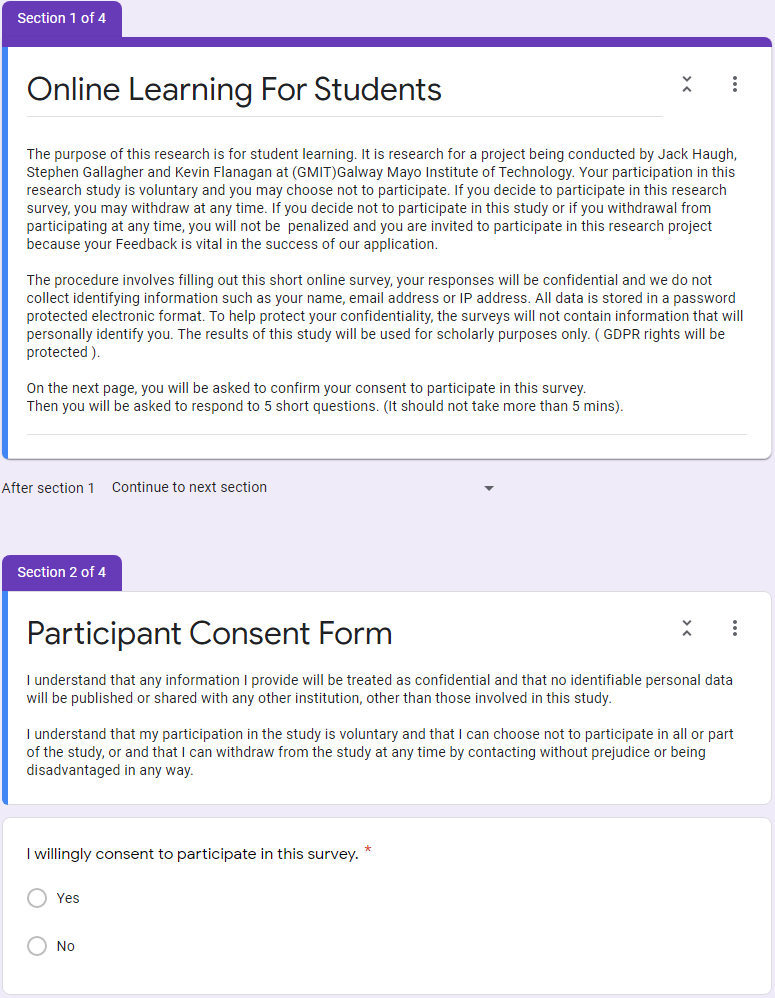
\includegraphics[width=6cm,height = 6cm]{images/22.png}
    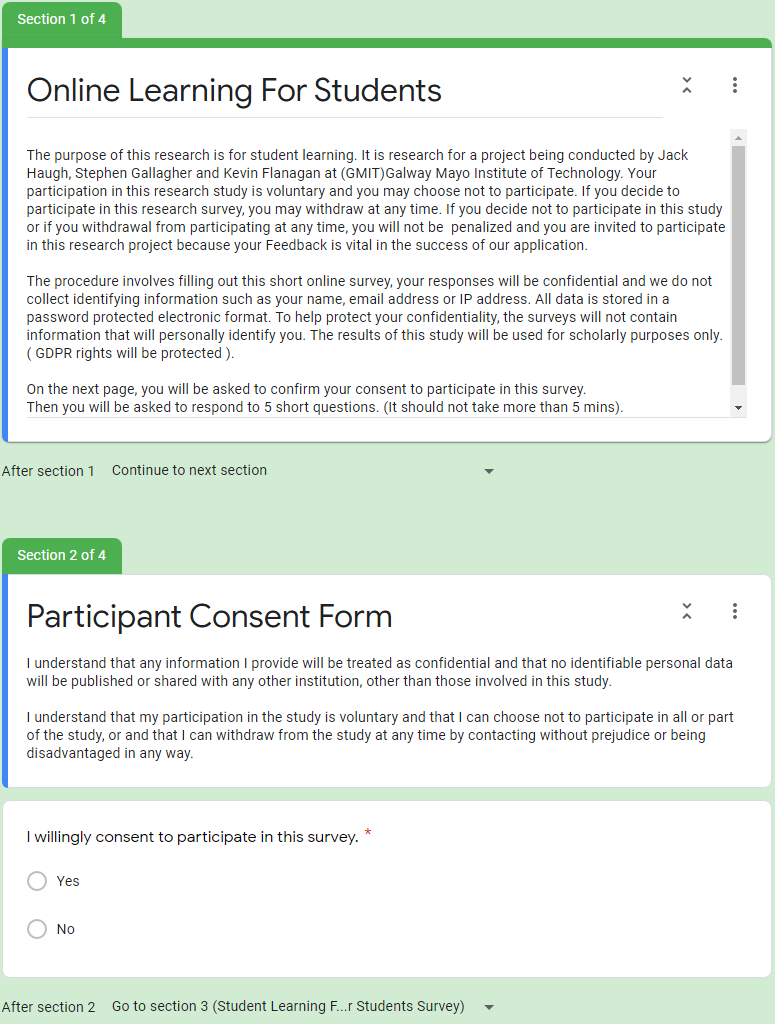
\includegraphics[width=6cm,height = 6cm]{images/23.png}
    \caption{ }
    \label{fig:my_label}
\end{figure}
Working on Google forms we will create these surveys and send them out to our fellow peers and see what feedback we can get. This feedback will hopefully lead us down paths that we wouldn’t have thought of ourselves and give us some insight into what people would like to have implemented into our website.
After deciding what we were going to ask (Questions below) students what features and what applications that they would like to see included and what would be helpful to their learning. Based on feedback we will be deciding on what we should be creating in our platform. \hfill \break
\hfill \break
We set up the two surveys on Google Forms, where we created a quick survey to gather information from students and other users with about 10 questions and some terms and conditions for the user to agree too. With this information we plan on adding or deleting different functions within our website and will give us an idea of what other students are looking for. The goal of this first survey is to hopefully come across an idea or function that we failed to see ourselves and if possible, to implement said function into our own site. The first survey we decided to email it to our peers and students in other courses to see what their responses would be to our survey.  \hfill \break



\begin{figure}
    \centering
    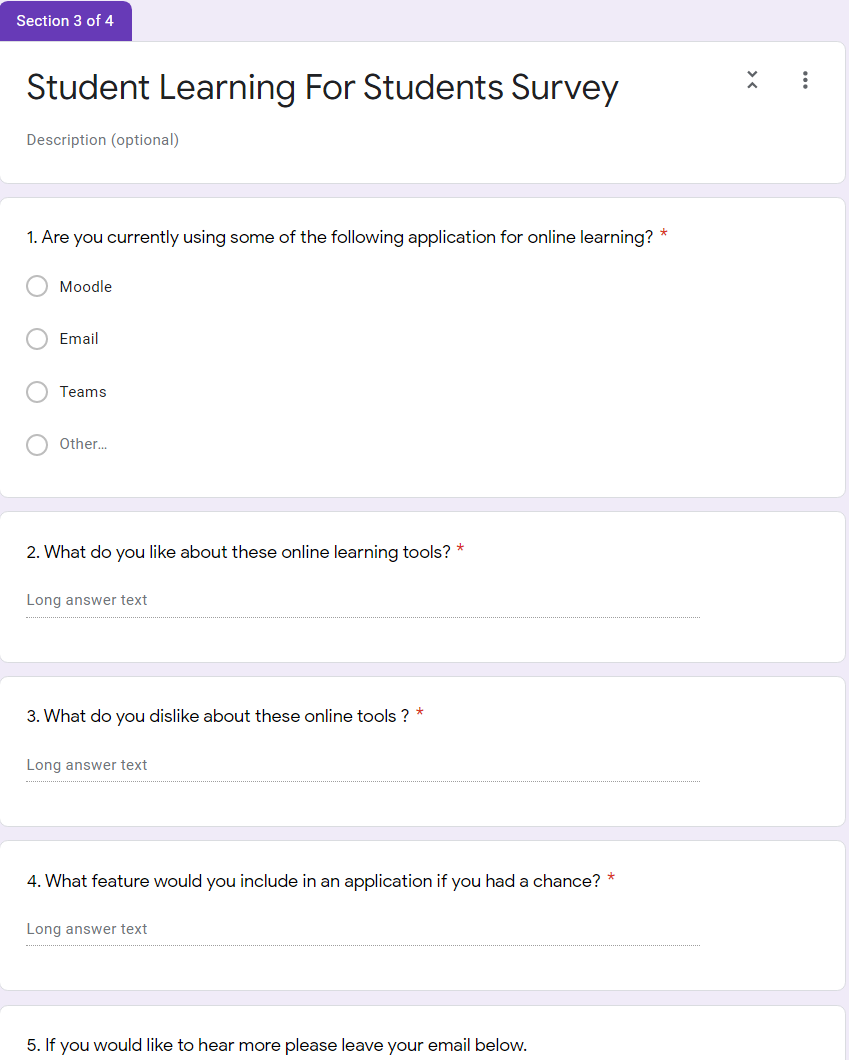
\includegraphics[width=6cm,height = 6cm]{images/24.png}
    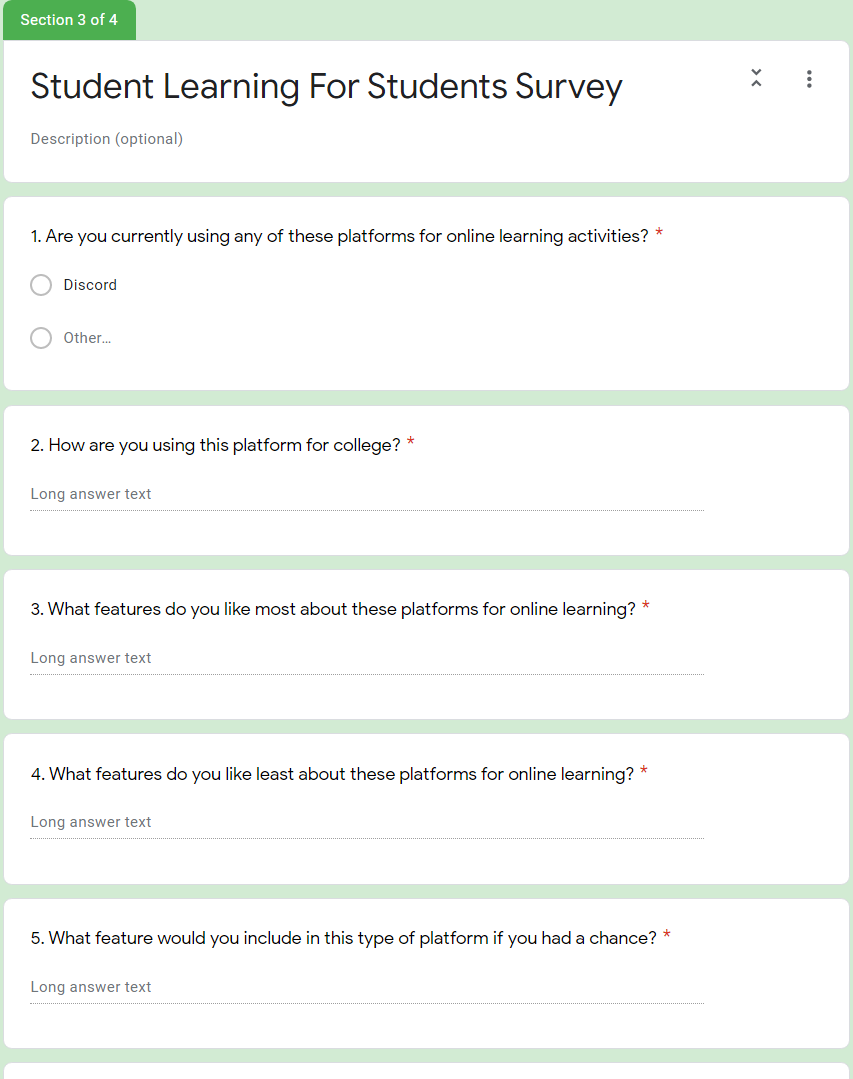
\includegraphics[width=6cm,height = 6cm]{images/25.png}
    \caption{ }
    \label{fig:my_label}
\end{figure}


The second survey we decided to be more specific in our questions, this will let us narrow down the possible results and answers that we receive back from the participants of the survey. Again, we are hoping to get that one bit of information or idea that we never thought of ourselves. For this survey we only needed 5 questions and they were aimed towards Discord which is a VoIP, instant messaging and a digital distribution website/app, from our first survey we discovered that this seemed to be the main way that students were communicating outside of college websites such as “Moodle”. This information let us narrow down the questions (5) we asked in our second survey and got a better view of what students wanted from this type of website/application.\hfill \break


\begin{figure}
    \centering
    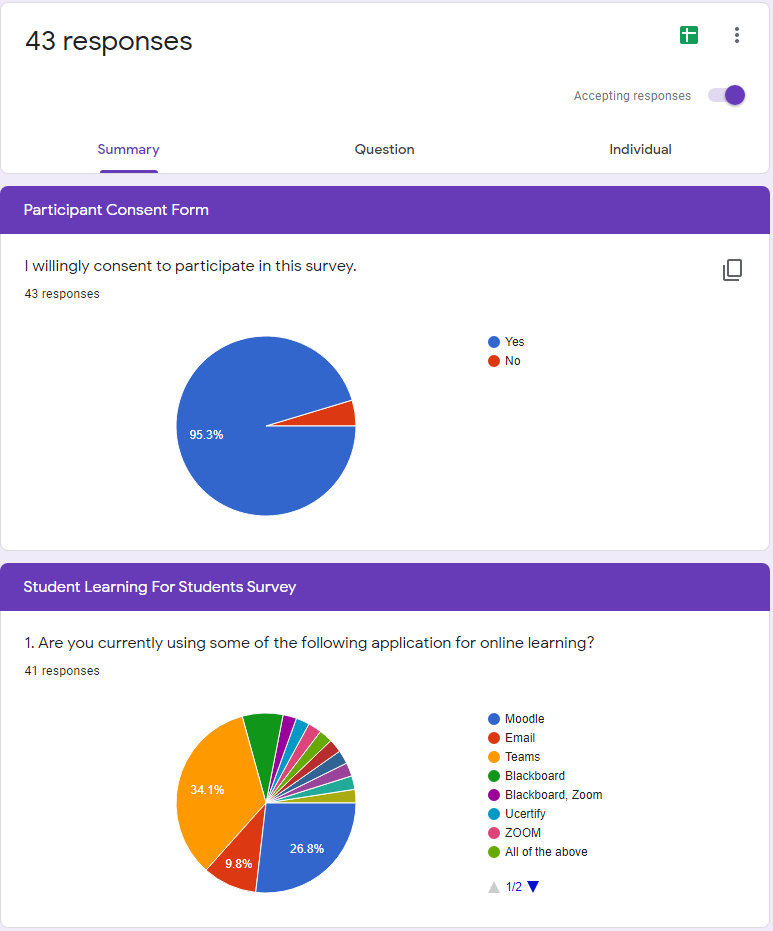
\includegraphics[width=6cm,height = 6cm]{images/26.png}
    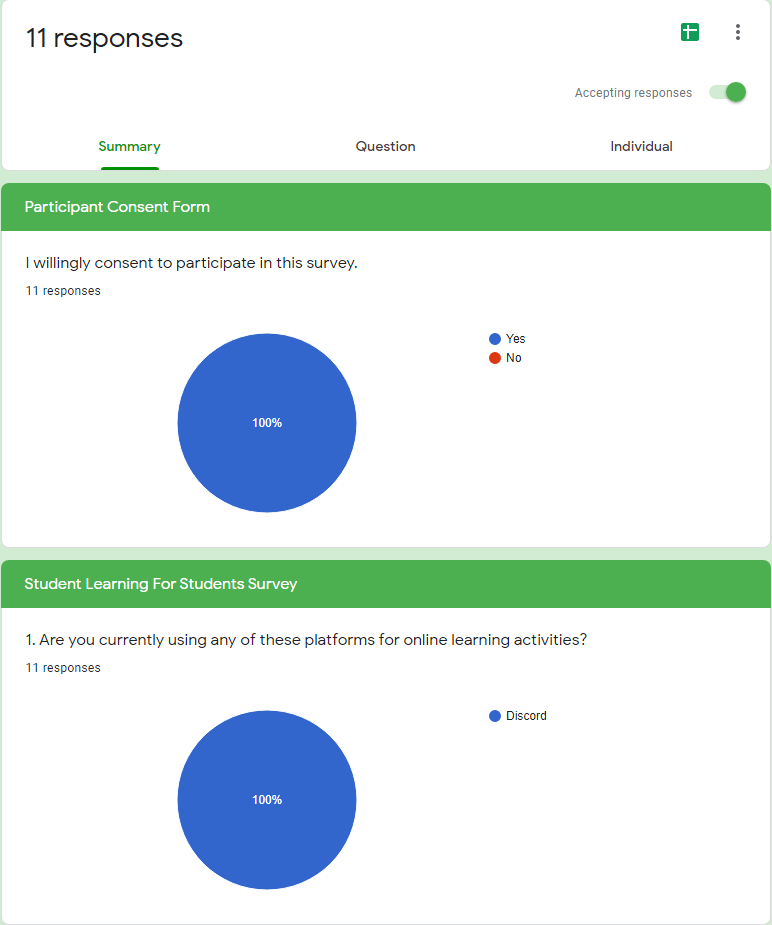
\includegraphics[width=6cm,height = 6cm]{images/27.png}
    \caption{ }
    \label{fig:my_label}
\end{figure}



With some great data gathered from the surveys from Google Forms\cite{ref26} we have a good idea what is expected in this type of website/app. From this information we hope to achieve a website/app that our fellow students would not only be happy to use be would also be helpful in their college workloads. 



\chapter{Methodology}
\section{Overview}
For our project, we decided to use the Agile methodology approach \cite{ref14} as we felt it what would be best suited for our project and our team. While also using agile we went down the route of adding the scrum\cite{ref15} technique to our project. Other points we have mentioned include the planning and meeting phase, time-management along with the version control we used throughout the cycle of this project.

\section{Agile Software Development}

Agile methodology is a product development framework that is consistent with the agile manifesto's standards and principles for software development. They want to produce the right product with small self-organized teams delivering bits of features at a time, listening to feedback, and fixing the product when it's supposed to be fixed. As a result, agile seeks to address the issues that people have had with the old and conventional ‘waterfall' strategy, which involves providing a large quantity of work over a long period of time and then having consumers change their minds during the process, wasting time and money. Teamwork and collaboration as a major step in product creation which can be really satisfying at the end stage because the team that has worked on this project and has fulfilled the targets set out by the customer at the beginning are the key features we found with the agile approach. Consumer input and communication are both important parts of agile, which we discovered during the months of progress on this project. We created surveys for feedback to hear from fellow students and see what they would like to see in a student application, hearing and getting feedback from the customer, or in our case, the students, is an important part of project creation.

\hfill \break

\begin{figure}
    \centering
    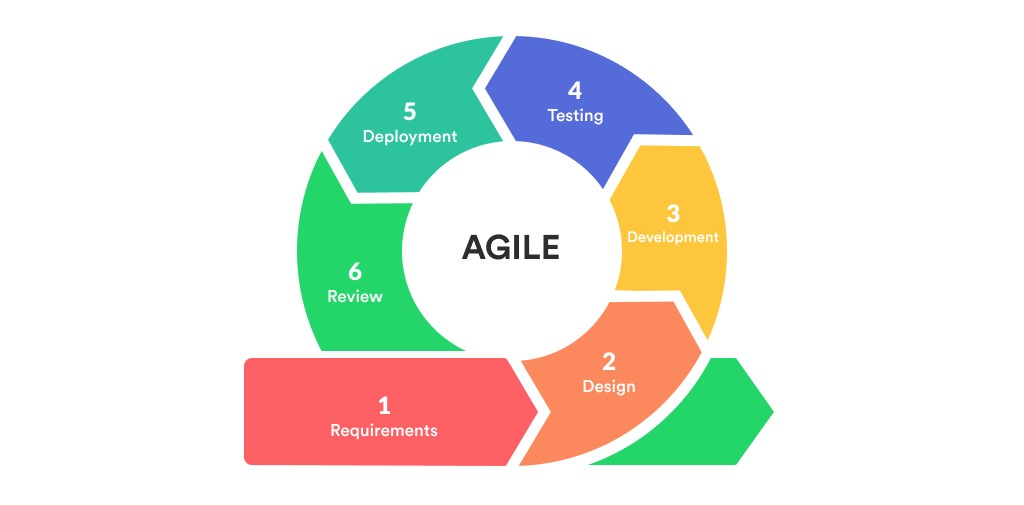
\includegraphics[width=.4\textwidth, inner]{images/87.jpg}
    \caption{ }
    \label{fig:my_label}
\end{figure}

\subsection{Scrum method}

We chose the Scrum\cite{ref15} technique as our key agile variant because we believe it best suits us as a team and how we built the project from the ground up and in the manner we did. We discussed what would be the right path to take for the day ahead, as we worked on the project as a collective at the start of our meetings. This was beneficial because it helped us focus on the key points we wanted to accomplish for the day so we could mark it off as a successful day. We didn't have many issues on the topics we set out to do on the day because we set the targets at the beginning with the emphasis on quality which was still top priority rather than concentrating on other tasks, which may have negative effects on the project. We also discovered that we invested our time wisely during the planning phase, and that the sprints we completed were effective and contributed to the project's success.

\section{Planning and meetings }

As fellow students, one of the biggest tasks we faced throughout our college cycle was to keep on top of the workload that we received each week from modules. For us to schedule what we were going to do with the project on various days. In semesters 1 and 2, we had weekly meetings with our supervisor Mark Campbell on Tuesdays, and we confirmed a day during the week to tackle the project, which normally fell on Fridays for ourselves. These meetings were well received by us because we felt Mark provided us with useful insight on how we were doing in the previous weeks and gave us structured input every week about what he thought would be successful additions to our site and was a big help to us along the way.\hfill \break

Trello\cite{ref9}, a web-based collaboration platform that allows users to organize tasks and boards/sticky notes, was introduced to us by our supervisor. It allows users to sort their boards into different sections and add boards to those sections, which we found very useful when we created a board called for example "Week 6 to-do" and added the boards to that section, and then when that board was complete, we created another section called "Week 6 done" and dragged the boards into that section as done to act as a checklist for us to know that we met the goals we set for ourselves for that specific week.

\begin{figure}
    \centering
    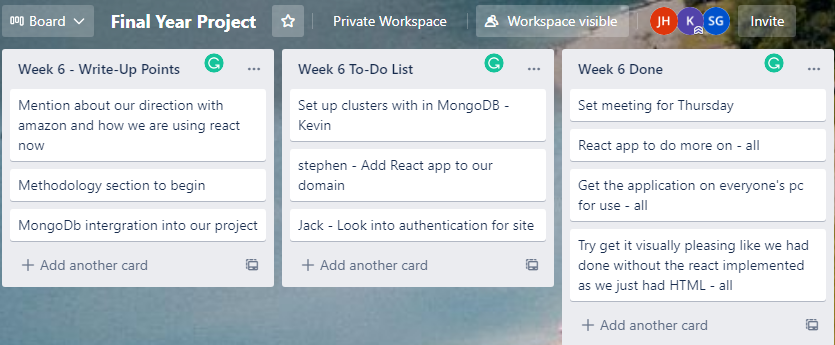
\includegraphics[width=.4\textwidth]{images/88.png}
    \caption{  }
    \label{fig:my_label}
\end{figure}



\section{Time-Management during project }

We all found that managing the workload for this project and other modules during our final year became difficult at times during the eight-month period of this project. Overall, with the inclusion of Trello and weekly meetings with our supervisor as well as meetings with ourselves, we were able to overcome many time-management problems and handle our workload very well. The use of our methodology, which included preparing our sprints during the year, greatly aided in the planning of the project's days and weeks. We believe that this project has also provided us with valuable experience, allowing us to better plan for our futures in this industry. We believe that this project has helped shape us for the long road ahead.

\section{Version control }
When we first began the project, we built a repository on Github\cite{ref5} and it's become a really important part of our project cycle since the beginning. It's a way to save our work by making regular commits that indicate what was completed and when it was done, as well as a great way to monitor progress across the course of the project. It allowed us to submit code from our project that we knew worked after completion and testing to our repository as a backup in case something went wrong. We also made adjustments that had an impact on the rest of the project and we needed to revert back to the code we knew worked previously. It has been and will continue to be an important tool for us to use in the future simply because of the consistency and value it provides to those working in this field.


\chapter{System Design}
\section{Research}
Based on our research a student will login and have access to their notes and timetable for there week ahead. All their classes and lab assignments will be displayed, and a forum will be added to allow students to ask their fellow students about any inquires or other questions they may have. 
Video calls would be a great feature to have within our application, the ability to talk and see your fellow students goes a long way in helping each other out when it comes to their workloads and will help in the social side of getting to know your peers. Part of college life is interacting with your fellow students and we think a feature allowing video calls would be a big step towards helping students in communicating. At the very least having a chat feature that students can use to communicate among themselves. 

Having decided on our project we have had a few meetings at this stage with our supervisor and have decided on breaking up the project between the three of us: 


\begin{itemize}
  \item Jack – WEBRTC the back end of the project and will use real time media communications. E.g. HTML5 
  \item Kevin – MongoDB setting up a database to allow information to be stored. E.g. Login details
  \item Stephen – Hosting and Frontend, the user interface that will be displayed on our site. E.g. Amplify , CSS files 
\end{itemize}

\section{Backend}


\subsection{MongoDB Key Features}

\textbf{Flexibility} - MongoDB\cite{ref17} was designed to work with cloud platforms and commodity hardware, data is then localized for queries that will ensure performance is at its peak no matter the deployment size of the project. \hfill \break

\textbf{Scale-Out} – MongoDB has been designed to be scaled across server clusters, when the data starts to grow, the user can add more nodes to the clusters and MongoDB will balance the data among the clusters evenly and automatically in the background. \hfill \break

\textbf{Dynamic Schemas} – This lets developers make changes that are required in the system without affecting the existing data already stored in the dataset, not incurring any downtime. With other schemas they must be defined before data is inserted. With MongoDB the schema is dynamic this allows it to be scaled as needed and supports fluent polymorphism.    \hfill \break

\textbf{Rich Querying} – MongoDB uses a full query language; a primary and secondary indexing is also used and a Google like text search.  \hfill \break

MongoDB is the perfect database to use within our project, with its flexibility, scalability and high performance using dynamic schemas this is perfect for our project. MongoDB is a document-oriented database that will allow us to store JSON documents with a dynamic schema that we will use to store our records/queries and will scale up as we need and also allow us to add or remove field and types as needed to our project. No other NoSQL or relational database software makes it as easy to use and to develop databases. 



\subsection{Hosted with Elastic Beanstalk}

We chose Elastic Beanstalk \cite{ref18} to host our database after some research as we discovered that it provides the best environment for us to host our database. Elastic beanstalk is the best fit for our application because it provides the same easy updating that Amplify\cite{ref22} does. We can update our frontend with Amplify whenever we want to push to our repository.
\hfill \break

Where with Elastic beanstalk when we run “eb deploy” it deploys the application source from the initialized project directory to the running application. Having both the frontend and backend so easily updated makes developing and hosting our application much less stressful, as well as saving time for any future development issues.
\hfill \break

We liked how Elastic Beanstalk saved time on configuration when we were researching it, but it wasn't just the time savings that drew our attention, it was also the way you can configure a custom domain for your Elastic Beanstalk environment, which we had already purchased from GoDaddy.com \cite{ref21}. Elastic Beanstalk allows you to use HTTPS to secure user connections to your application.
\hfill \break
\hfill \break
Overall, we could only see the advantages of using Elastic Beanstalk because it provided an easy setup with great benefits, similar to what we experienced when we switched our frontend to Amplify.



\subsection{Elastic Beanstalk troubleshooting Issues}


During the development of our application, we ran into a few roadblocks that necessitated additional research or troubleshooting. This section demonstrates our thought process as we attempted to resolve the issues we encountered with Elastic Beanstalk, as well as how it led us down the path to resolving these issues in subsequent sections.

\hfill \break
\large
\textbf{Error with instances:}

\hfill \break

\textbf{Step 1:}\hfill \break
we tried going through each section and trying to narrow down the issue we were facing with Elastic Beanstalk.\hfill \break

\textbf{Step 2:}\hfill \break
We started off by checking if the instance is running "ok" in general.\hfill \break

\textbf{Step 3:}\hfill \break
We noticed there was no Elastic IP addresses assigned which made us research further, to see if it was required for the traffic through the application.\hfill \break

\textbf{Step 4:}\hfill \break
We started looking into VPC which is a Virtual Private cloud that allows you to control who has access to your AWS resources,as we noticed on the following website.\hfill \break

\textbf{Step 5:}\hfill \break
When setting up the environment on AWS you have the option to select VPC or load balancer. This will let the Hosting service balance the load for you and allow you to add extra instances, but you can make the visibility public.\hfill \break

\textbf{Step 6:}\hfill \break
We researched the sections on YouTube\cite{ref23} for more of an understanding into VPC on AWS. \hfill \break

\textbf{Step 7:}\hfill \break
We took note that our Network on our environment was not part of a VPC.\hfill \break

\textbf{Step 8:}\hfill \break
We Looked online for videos and came across the way in which to find the load balancers IP addresses. These addresses we added to MongoDB to see was it an access problem. \hfill \break

\textbf{Step 9:}\hfill \break
We researched a video to complete a walk-through of Elastic beanstalk and linking the domain with the database through HTTPS. Which we believed to be for security reasons.\hfill \break

\textbf{Step 10:}\hfill \break
We then went onto Requesting a certificate for our domain.\hfill \break

\textbf{Step 11:}\hfill \break
After requesting a certificate we researched how long it would take for a certificate to be issued by AWS and it was up to 48 hours.\hfill \break



\hfill \break
\subsection{Elastic Beanstalk HTTP issue overcame}

\hfill \break


\textbf{Step 1:}\hfill \break
we added route 53 CNAME for HTTPS certificate.

\textbf{Step 2:}\hfill \break
We added to route53\cite{ref20}, it can take up to 30 minutes for the change to process and for AWS to validate the domain we have setup.\hfill \break

\textbf{Step 2.1:}\hfill \break
After we allocated time, route53 had been updated.\hfill \break

\textbf{Step 3:}\hfill \break
After this we went and checked what listeners had been assigned to the load balancers. By default you can see that you have HTTP:  on port 80 .\hfill \break

\textbf{Step 4:}\hfill \break
We wanted to change it to HTTPS listener on port 443. As we don’t want unsupported traffic running to our servers, we first checked if our certificate was issued. \hfill \break

\textbf{Step 5:}\hfill \break
We changed the http to Https.This we found will only appear when you have "CNAME" defined on Route53 and while the certificate is issued.When the certificate is issued we then were able to select the HTTPS as a listener at the bottom of the new port 443.\hfill \break

\textbf{Step 6:}\hfill \break
we then confirmed our changes.\hfill \break

\textbf{Step 7:}\hfill \break
After the updates were completed we were then issued a warning, this told us that the port was not receiving traffic.\hfill \break

\textbf{Step 9:}\hfill \break
We had to check in the security group to see what ports it was using for access.\hfill \break
 
\textbf{Step 9:}\hfill \break
We changed  the inbound inbound rules to allow traffic on https.\hfill \break

\textbf{Step 10:}\hfill \break
Confirmation of change confirmed HTTPS working for our application now (fixed our HTTPS Issue as now no longer stated as an issue)\hfill \break



\hfill \break

\subsection{Elastic Beanstalk failed on all instances overcame }

\hfill \break
\textbf{Step 1:}\hfill \break
Requested the last one hundred lines of the logs so that we could see where the error is coming from.\hfill \break
\hfill \break
\textbf{Step 2:}\hfill \break
Noticed it was a 111-connection upstream error \hfill \break


\textbf{Step 3:}\hfill \break
We Researched the error on google and multiple forums

\begin{itemize}
  \item Came across some people saying it was a dependency issue with their app and AWS(which was a different type of application)
  \item Others were saying it was a connection issue between AWS and the application.
\end{itemize}

\textbf{Step 4:}\hfill \break
We double checked what happens when we run the environment for AWS.\hfill \break

\textbf{Solution:}

The only solution to fixing the severe health issue with our elastic beanstalk was to “Rebuild” the environment. We tried to avoid rebuilding our environment as this would have consumed too much of our time when we could allocate it to meeting other deadlines.
After “rebuilding” the environment and making the necessary changes to the following

\begin{itemize}
  \item The load balancer.
  \item Route53.
  \item Applying for the HTTPS certificate. 
\end{itemize}

We were delighted to announce that the rebuild had worked and that Elastic beanstalk\cite{ref18} had gotten confused somewhere along the way.



\section{Frontend}
\subsection{AWS (Long approach)}

\textbf{HTML and CSS files to AWS amazon} - When setting up the application to be hosted by AWS amazon we had no prior knowledge behind the hosting service. This resulted in us to doing extensive research into the hosting providers.\hfill \break


We had to research the following before uploading anything: S3, Route53, EC2. These areas of the hosting providers we found vital in achieving what we would need from Amazon’s web services.\hfill \break


To begin we researched S3 buckets \cite{ref19}. After a few posts and videos, we became aware that it is Amazon’s way of storing files. Our understanding at the beginning was limited to seeing just files but after doing some more research on the subject we could see that the user could restrict access to these files. We learned that this is used to protect the access of the files which can be retrieved from anywhere on any device through the web if needed. \hfill \break


Following this research, we began looking at Route 53, we started to understand that this would be needed for directing the files that would be uploaded. Route 53 being Amazon's widely available and scalable cloud domain name system (DNS) service. From this research we learned how it helps host your files to the web for the public to see on any browser worldwide.

\subsection{AWS Long approach issues overcame}

When initiating the implementation of our research we came across some difficulties and roadblocks, with the S3 buckets. There were a few more secret configurations that needed to be updated in order to complete the task at hand. The two issues we had with Amazon's S3 buckets were that we didn't realize you had to allow permissions on them when we uploaded all the files for the application. This allowed users to have public access to these files. To be able to see the files on the web, we had to make them static while also selecting to unblock public access.\hfill \break


Route53 appeared to be for routing at a first glance, but we had no idea what was required. After conducting extensive research, this became clear. After watching videos and participating in forums, we realized what was needed.
This included a "Record A," which maps the URL to one or more IP addresses when the IP is known and stable. 
The "record A" points a name to a specific IP. For our application we used the alias target that amazon provided us with. This saved us from looking up the IP address of the domain. It is by default that Amazon gives you a hosted URL.

A "record SOA," which is the authority record that identifies the domain's "DNS" information, was also required. It keeps track of important details about a domain or zone, such as the administrator's email address, the last time the domain was updated, and how long the server should wait between refreshes. We discovered that in order to comply with "IETF" standards, all "DNS" zones require a "SOA" record.

What was also needed was what Amazon provided by default. The name server "NS" record. Once the user created a hosted zone, the name server record is created. It contains a list of the four authoritative name servers for your hosted zone. They advise against making any changes to these name servers. 

A “CNAME” record was the final requirement that we needed to complete our Route53. This record was required for mapping of our Amazon's default URL domain to www.Student-mania.com, which we purchased on GoDaddy.com.


\subsection{AWS Amplify (Short approach) }

\textbf{HTML & CSS & JavaScript & react to amazon aws amplify} - Uploading to amplify we discovered that we can only host the application to amplify if we were the admin holder of the repository of the project. We soon uploaded the project to amplify but came across some issues. Where we wanted to be able to contact customer support but due to them removing the live chat functionality unless you pay for a plan, we were unable to access this feature. We then had to research why we were getting the error “page cannot be found error 404”. We knew this to be a linking issue as it was there but couldn’t be located. After extensive research we failed to find the solution, We discovered that this was not sufficiently addressed in online discussions or in any of our other research, which yielded no findings.\hfill \break

The solution we found was that when you are uploading to AWS Amplify and linking your repository to it, the user must click on the small box at the end that allows the admin to specify the exact folder of the application within your repository folder. This is not covered or explain to be “needed”, when we were going through the process. We thought this was an extra feature, but between trial and error we figured that this feature needs to be ticked to declare the primary “my-App” as the repository folder.\hfill \break

We also discovered when we were researching, we came across that when you are uploading the repository to Amplify that when Amplify discovers your application and it looks for your “package. JSON” file. This then tells Amplify all the commands required that are needed to build the application.
Once we got round the issue of error 404, we had the application hosted by AWS Amplify as seen running through the deploying stage of Amplify.\hfill \break

\hfill \break
During the second way we were trying, it was unfortunate that Amazon started to set up plans for users to have to pay for help off customer service, if a user wanted help in other ways than live chat they would have to sign up for a plan. This feature which we used at the end of the first way of going about uploading the application website to AWS Amazon. As after we uploaded everything, we were still unable to see the website but on live chat we were helped out within minutes. Being explained to us that it could take up to 48hrs to fully upload and be visible on the web with the URL they provided.



\subsection{Linking Frontend AWS Amplify with GoDaddy Domain}

In our learning and researching of linking our domain to Amplify we learned that when you setup a Route53 it provides you with the four name servers and "SOA". When you go to your “Domain management” section on your AWS Amplify and select the Route53\cite{ref20}, you must proceed to setup the two generated fields, “CNAME” and “ALIAS(A)” that amplify provides for you. This which had to be done manually when not using AWS Amplify.


Since we have hosted now both ways using AWS, we now know specifically what Amplify does for its users, so they don’t have to setup everything themselves which can make the setup very convenient and less time consuming for new users.\hfill \break

In the process of adding our custom servers to our GoDaddy domain we ran into an error when we clicked the save button. This error which was “an unexpected error”. When we looked up this error it came back to be a common error with GoDaddy.com. This suggested to access it on an incognito window or clear the user’s cache. This process did not work for us and we ended up having to contact customer service via live chat.\hfill \break

We were extremely happy to hear they had live chat but unfortunately the customer service person did not provide us with a reason behind the error. The only solution was that he entered the name servers for us into our account and then save it. We found this to be very strange but decided to try the same thing again but under a different name but got the same results and got the same error. After all the issues by the end of the day we were happy to say we got the website up and running and reachable through google for the second time using a different hosting method under the same provider.\hfill \break

Amplify is very useful when making changes to your application as you don’t need to re-upload your files to your S3 bucket\cite{ref19} to update your online application. It simply automatically rebuilds your application when you make a change/commit to your linked GitHub repository. This which saves time and helps in faster development of applications.

\section{Help page}


We setup a walkthrough/help video for users in case they find themselves for any reason lost on our application. This help page that will provide them with a place to go and watch a video that they can get a tour throughout the entire application while listening to soothing music in the process.
To make the video, we used Adobe Premiere, a video editing software that can produce high-definition videos with a lot of features, and we added soothing background music to make it more inviting and enjoyable to watch. We added text to each section of the video so that the user could understand why each feature on each page of the website was implemented.
We then uploaded the video to YouTube, which is one of the world's most popular video sharing platforms, with billions of users every day. Hosting it on YouTube\cite{ref23} also allowed us to use it as an embedded video to use as a source within our website.
Having a walkthrough/help video made and available to our target audience allows for less confusion if any arises, as well as getting our application out there on the web as another form of social media strategy for getting our logo seen.
After watching our video, we hope that no user will have any questions about the application's layout.

\section{WebRTC}

WebRTC\cite{ref16} will enable us to use audio, video and share data communication between browsers without having to use any plugins. This will allow us to simplify communications on our website and will also improve the users experience while they are logged into our website. After becoming available in 2011 WebRTC has only grown in popularity with an estimated 2 billion browsers that are enabled to use WebRTC. WebRTC is an open source project that can be customised as the developer sees fit, it is also completely free to use and is constantly evolving and improving over the years.   
ZOOM and Facebook messenger are two of the biggest names in the industry that use WebRTC to help improve their products. 

\section{Chat page}
\subsection{Chat engine}


We used a chat engine\cite{ref24} to create our chat page. This is an object-oriented framework for creating JavaScript chat applications. We selected chat engine because it drastically reduces the time it takes to build chat applications and includes essential features such as type indicators and the ability to create chat rooms, which are ideal for the purpose of our chat page.
By importing the chat engine system into our project, we were able to use all its features, which provided us with all the components we needed for students to communicate and exchange thoughts and notes on a regular basis. Students considered sharing their problems and files over applications to be beneficial and a faster way to resolve issues in our experience.
We found the documentation to be very helpful in setting up the chat engine because it was very clear and understandable, which helped us to achieve the goal of our project and provide our future users with the communication aspect we aimed for our chat page



\section{User story}


\textbf{Step 1:}\hfill \break

Login

\begin{itemize}
  \item User gets initially displayed with login screen when accessing www.student-mania.com
  \item User must register if they haven't created an account
\end{itemize}
	

\textbf{Step 2:}\hfill \break

Prompted to home (after login)

\begin{itemize}
  \item Can access any of the navigation bar options
  \item Home screen has a carousel with what the application offers
\end{itemize}

\textbf{Step 3:} \hfill \break

The navigation bar options for the user

\begin{itemize}
  \item  “Home” – to bring user to homepage
  \item  “Contact Section” – Help page, Query page, Forum page
  \item  “Resources” – Covidfaqs, Tweets, Sports, Useful software
  \item  “Social” - Video chat
  \item  “Student-Mania Chat” – Instant messaging and file sharing
  \item  “Logout” - Go back to the login page
\end{itemize}


\textbf{Step 4:}\hfill \break

 Help Page
\begin{itemize}
  \item Video to give tour around the website for users if needed
\end{itemize}


\textbf{Step 5:}\hfill \break

Query Page
\begin{itemize}
  \item Ask a query
  \item After the submission the user can go to the forum page by clicking the button which prompts them to the list of posted queries
\end{itemize}


\textbf{Step 6:}\hfill \break

Forum Page
\begin{itemize}
  \item See all displayed queries that have been posted by users
  \item Can see three buttons that guide the user from the list of questions, Go to query page to create a question, Reply via our applications chat for instant peer to peer or Get prompted towards our "Linktree"\cite{ref30} page where you can access any of the email communication platforms of the users choice in order to reply to a user’s question by email
\end{itemize}
  

\textbf{Step 7:}	\hfill \break

Covid fAQs Page

\begin{itemize}
  \item Helping students keep up to date with the current pandemic and keeping them aware with page that directs them to the HSE website if needed.
\end{itemize}


\textbf{Step 8:}	\hfill \break

Twitter Page

\begin{itemize}
  \item Let students see what the current day to day news is from all educational institutes from around the country
\end{itemize}


\textbf{Step 9:} \hfill \break

Sports Page

\begin{itemize}
  \item Access the different educational institutes sports teams 
  \item Keeping up to date with all sports
\end{itemize}



\textbf{Step 10:} \hfill \break

Useful Software Page

\begin{itemize}
  \item  Software recommended for students to make their everyday tasks easier
\end{itemize}



\textbf{Step 11:} \hfill \break

Chat Page

Allows users to do the following:

\begin{itemize}
  \item Send files
  \item Send messages
  \item Share notes
  \item Discuss classes
  \item Create chat rooms
  \item Choose who’s in each chat
\end{itemize}



\textbf{Step 12:} \hfill \break

Webcam Page

\begin{itemize}
  \item Create a room 
  \item Start sharing your webcam and microphone
\end{itemize}


\chapter{Technology Review}

\section{Authentication}
\subsection{Firebase}


Security and authentication have been a major factor for the user's online experience to store personal details such as names, addresses, and bank card information for any website or application in this period. We decided that our website required a login/registration authentication so that people could access and use the features on our website. We first learned about \textit{MongoDB Realm \cite{ref28}} and considered using it for our authentication but found it difficult to incorporate into our website due to our code and \textit{MongoDB Realm} not working together, so we abandoned the idea. We then chose to use Google's Firebase\cite{ref27} authentication after further testing and research.\hfill \break

Firebase is a Backend-as-a-Service provider (BaaS). It provides developers with a variety of tools and services to help them build high-quality applications, expand their user base, and grow their profit. It is built on Google's infrastructure. Firebase also has a NoSQL storage service that uses JSON-like formats to store data. Google's mobile platform, Firebase, makes it simple to build high-quality applications and will be a great help in developing your project. To authenticate users to your software, Firebase authentication offers backend services and ready-to-use UI libraries.\hfill \break

On our website, we have a login/register section where users can create an account in order to access it. If you don't add an email address or enter a password that isn't long enough, the signup is set to not allow the user to proceed, sending you messages like "The email address is poorly formatted.", if you don't add an email address or if you don't enter a long enough password "The password must be 6 characters long or more.". If the user goes to login after creating your account and the email address is incorrect, it will give you a “The email address is badly formatted.” message, and if the password is incorrect, it will give you a “The password is invalid or the user does not have a password.” message, which we believe is required for every site to let users know the status of their account.\hfill \break

The code we used for this started with the class ‘fire.js,' which was provided by Firebase when we developed the project online, which acts as a conversation between the login/register and the storage online, as there are API keys to communicate with the site online. The following two classes, ‘login.js' and ‘app.js,' work together to allow users to login and register for access to the website. The ‘login.js' class has variables for storing emails and passwords to send to the Firebase API\cite{ref27}, as well as handling email and password errors. On our login/register section of the website, we have input boxes setup for the user to sign up or login to the website, and we have it setup to also handle sign-up and login errors here if the user enters incorrect information.\hfill \break

The next class, ‘app.js,' has consts for user, email, password, emailError, passwordError, and hasAccount, all of which are empty strings, so they take in the data and check it against the username, if an account is already created or registering for the first time. The first method is 'handleLogin,' and here is where it checks with the fire.js class to see if the information is correct and identical to what is stored in our database. It also has a switch statement for errors such as invalid email or user not identified, as well as a switch statement for incorrect password.\hfill \break

The second feature, ‘handleSignup,' tests with the fire.js class to see if the information entered is brand new, allowing the user to build a new account. There's also a switch statement for errors like an email address that's already in use or an incorrect email address, as well as whether the user enters a password that's less than 6 characters long. It also has a ‘handleLogout' method that allows the user to log out of the website after visiting it by informing Firebase that they have done so. The final method is 'authListener,' which tests whether the user's details are correct and whether the user exists when retrieving the information from Firebase.\hfill \break

We all agreed that security is a must for people visiting our site because security is a top priority in today's world of online browsing. For the sake of our clients' peace of mind, we wanted to make sure that their personal information remained confidential and safe on our website. Overall, we were pleased with our Firebase research for our project, and we believe it adds a critical security element to the development of our application. We agree that adding a login function that interacts with social networking accounts such as \textit{Facebook, Twitter, and Google} will be a welcome addition to the application for potential growth, as it would encourage increased connectivity amongst users.


\begin{figure}
    \centering
    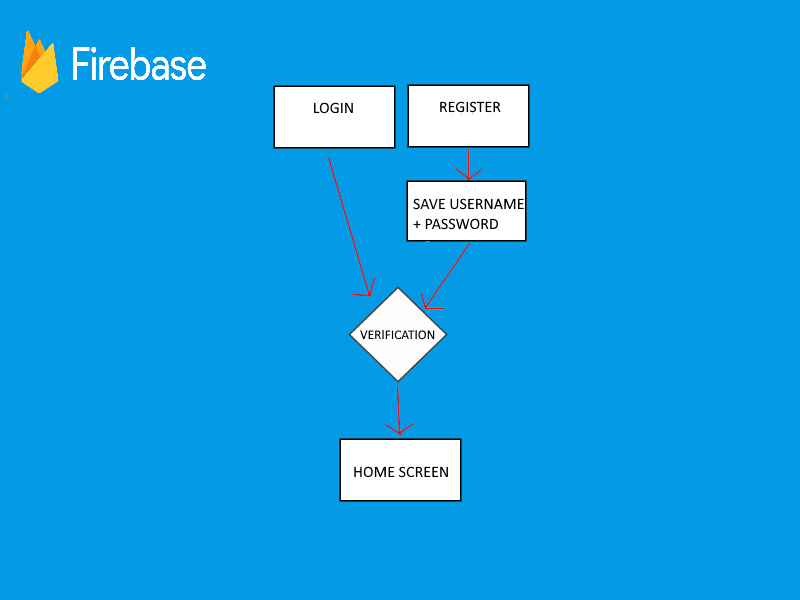
\includegraphics[width=6cm,height = 6cm]{images/45.png}
    \caption{ Firebase Diagram }
    \label{fig:my_label}
\end{figure}

\section{Databases}
\subsection{MongoDB}


The front-end has been created with a great display and very user friendly. We plan on having our website hosted globally and have our databases and servers running with a GoDaddy\cite{ref21} domain letting it be accessed from anywhere. The next biggest step is to set-up MongoDB to be our database for the website to store details and secure logins. This will allow students to share documents and notes from lectures and classes, forums to ask questions, Video calls with fellow students. \hfill \break  

MongoDB is an object-oriented, dynamic and a scalable NoSQL database that stores information in data objects. These data objects are then stored as separate documents inside of a collection. These collections are created by the user and then a cluster is created within the collection. \hfill \break


From the image above we had to connect the cluster to our application which involved a line of code, that would allow our website/application to connect to the database to write and share information while also saving it to the database to be recalled when server is running. To allow MongoDB to receive information from the website/application while also returning the information when called upon in the future we created a database called "modulesDB" which had collections that will store information that is desired for the different sections of our website/application. We then created different classes within our directory that “talked” to each other to send and receive information. This information is needed firstly to receive the information from the user and then secondly to return that information to be displayed for all users to be seen on our website/application.   


\begin{figure}
    \centering
    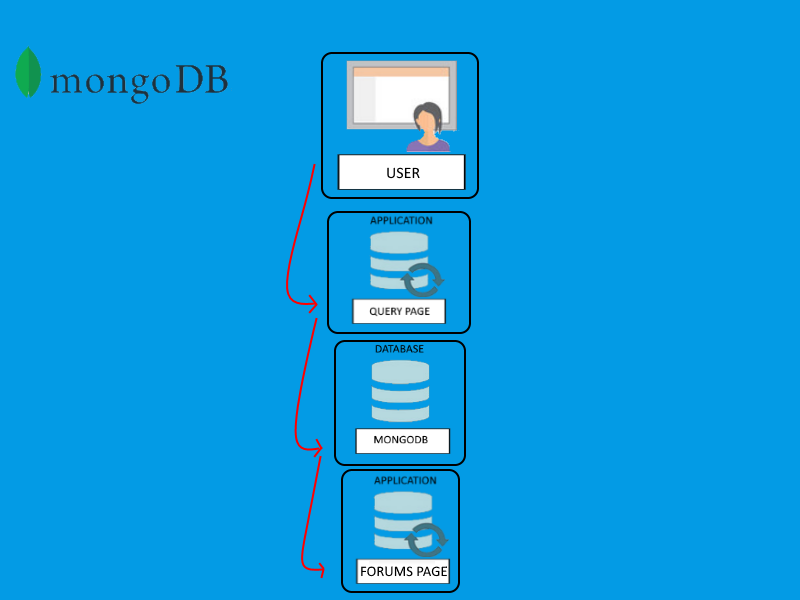
\includegraphics[width=6cm,height = 6cm]{images/28.png}
    \caption{ MongoDB Diagram}
    \label{fig:my_label}
\end{figure}


\section{WebRTC}

We had the idea to incorporate a webcam feature into the site during the planning process because it would be a perfect way for students to interact with their peers and fellow students. That's where we discovered WebRTC, a free and open source project that allows web browsers to communicate in real time via application programming interfaces. \textit{Facebook Messenger, Discord, HouseParty, and Google} are some of the larger applications and companies that use webRTC. \textit{Google} is a major supporter of webRTC, since they were the first to introduce the technology in 2011. Google hangouts/meet was developed as part of Google work-space and became their prime video conferencing technology.\hfill \break

WebRTC has been a big hit with companies and developers across the globe since its release for many reasons. Since it is an open-source software, it enables end-to-end direct communication and a faster and simpler link between browsers such as \textit{Google Chrome, Mozilla Firefox, and Opera GX} without the use of a third-party application. This eliminates the need for additional applications and plugins while also offering a much safer and secure application. \hfill \break

We plan to use peer-to-peer networking on our application and this would allow more people to participate in the video chat at the same time. As a result of our viewing of tutorials and documentation, we found it difficult to implement the peer-to-peer connection because it wasn't working as planned, it allowed one person's webcam to display but sending the URL link to invite your fellow peer wouldn't enable them to participate within the call, even with the videos we watched, they never had any trouble developing their application and made it look easy. \hfill \break

According to the code we implemented, it begins with a class named ‘CreateRoom.js' that has a button called create room that, when pressed, redirects the user to a created room with a random URL that they can then send to a fellow user to enter the video call. We then proceed to the ‘Room.js' tab, which contains the methods for managing the various aspects of the video call. If the user acknowledges the browser's permissions to use these functions, the useEffect method allows sound and video to be played on the computer. \hfill \break

The callUser feature allows a user to send a connection to a peer and have a video chat with them. Through creating the link, the createPeer method establishes the connection with the person you're trying to call. By targeting the other peers' userID, the handleNegotiationNeededEvent method takes care of the userID setting up the link for the call. The handleReceiveCall method takes care of the peer who receives the call by going through various lines of code to approve it, as well as the user trying to connect. When the user answers the call, the handleAnswer method transfers the RTCSession variable to the code, telling it that a call has been answered and is in progress. From here, the user can enter a room by selecting “Social” from the drop down menu in our navigation bar, then build a room by selecting the "Create Room" button, and then give the user the connection to their room, where they can join and talk one-on-one.\hfill \break

We thought this feature would be a positive addition to our website, allowing students to make video calls to one another, given how important voice and video chat has become in the year since the global pandemic began. If students can make voice and video calls to their fellow students whenever they want, they will be able to get work done and receive help from anywhere with a connection. When students are removed from their normal learning environments and need to complete assignments in classes or in group assignments, this gives them a lot more versatility when it comes to time-management by meeting deadlines. Video calls can be a great motivator to get work done by talking with each other through computer screens rather than hearing each other's voices, and this provides a new way to learn and socialize in this modern age.\hfill \break

We hope to add peer-to-peer or possibly one-to-many connections to the website if we return to work on this topic because we believe it is an integral part of the website for future use, as we have seen during the recent global pandemic how important this technology has been for the world.


\section{Font Awesome}

We used Font Awesome\cite{ref29} website to get icons that we could use to link our social media accounts to our website for advertising and easy access. This makes navigation between the social media accounts easier for the users.
To use these icons on our website we had to make an account that provided us with HTML code that we had to have embedded in our code to allow the icons to appear.
This after having embedded in the body of my code which allowed us to search for icons on the website. There we selected the one we wanted, and it then provided us with more HTML code that we simply had to paste into our application where we wanted it to be displayed. Here where we embedded this HTML code from the website into a href tag that allowed us to reference a website when a user clicks on the icon. This we repeated for each social media account that we wanted to reference.




\section{Linktree}

This website we registered with to allow us to link multiple websites to the one account within our application. This makes it easier to list to the users the accounts all in one place in an organised fashion. We had to sign up using an email account to verify the email. Here we created the account under the username of the application called Student-Mania. We concluded that this was the best option for future expansion when multiple websites will be created for marketing purposes for addition to our application. The application's intent and functionality were fulfilled by including this.


\section{Twitter integration}

\subsection{Twitter Publish.twitter.com steps}

\textbf{Step 1:} \hfill \break
This website which allows a user to enter the twitter account of their choosing and be provided with the embedded HTML code to paste into their website. This code then displays the twitter feed from the respected twitter account chosen.\hfill \break

\textbf{Step 2:} \hfill \break
After the user selects the account the user can then chose which way they would like to display the account feed on their website with two options. (1) Embedded timeline or (2) Twitter buttons.\hfill \break

\textbf{Step 3:} \hfill \break
Then the user can customize the feed to their liking. This can be by size, width or even colour.\hfill \break

\textbf{Step 4:} \hfill \break
This wouldn't display correctly when added to the HTML directly into the React application. This required the additional code to run correctly.To install the dependencies for the Twitter feed to display in a React application.\hfill \break


npm install --save react-twitter-embed \hfill \break

\textbf{Step 5:} \hfill \break
To import these dependencies to the HTML \hfill \break

import { TwitterTimelineEmbed, TwitterShareButton, TwitterFollowButton, TwitterHashtagButton, TwitterMentionButton, TwitterTweetEmbed, TwitterMomentShare, TwitterDMButton, TwitterVideoEmbed, TwitterOnAirButton } from 'react-twitter-embed';\hfill \break

\hfill \break
\textbf{Step 6:} \hfill \break

To add the following tag to display the feed on the page \hfill \break
"TwitterTimelineEmbed" \hfill \break

This which allowed us to display multiple twitter feeds on the application.




\section{Social media accounts}
\subsection{Facebook}


We created a Facebook\cite{ref10} page for users to discover our application. As Facebook allows more than two billion users to come across new applications daily. Setting up a Facebook page for the application helps with social media marketing. Social marketing is very important for new upcoming applications as it improves the awareness and and can increase the flow of inbound traffic.\hfill \break

We wanted to create more awareness to our application by social media accounts as we researched into social media strategies and what it takes for a application to be recognised. We discovered that it takes between 5-7 times for a brands logo to be remembered. This when posting daily and weekly we will help improve the recognition and flow of users onto our application in the future.\hfill \break

We also researched a business plan that Facebook provides, called "Facebook Business". As you can see from the image below at the start of our project we completed the basic steps working our way up. This involved creating our page and posting our very first Facebook post. \hfill \break

You can see from the image on our website, Facebook also allows the page owner to “boost Post”. This is a feature that also helps people to get their brand/application out there into the public eye. It is a feature that Facebook have implemented that requires a money plan option that “Boosts” the post so it will show up in your audiences news feed as an ad.
Facebook provides an easy use display where the Facebook page owner can select the "duration" and the "end day" of the boost while also stating their budget. Facebook will take all of this into account and respond to the page owner depending on the number of potential customers they will reach with their ads each day.\hfill \break

When setting up the Facebook page and researching the social media strategies we became aware that in 2012 that Facebook in fact bought another social media platform called Instagram for 1.0 billion. This we found great as we also noticed that when boosting your post Facebook allowed its users to select Instagram as an add placement for your post too.
Here we Realised that having the two platforms reaching as much of our target audience would be very beneficial and began to move onto Instagram also to broaden our reach.


\subsection{Instagram}


We launched straight into making our Instagram page after creating our Facebook page as we now know the benefits of reaching our target audience and getting our applications name out there for people to see. Having another social media account helps us as a team connect with our audience through the stories and posts that we can create, this make our application relatable and express how user friendly it is.
Instagram also provides a feature that makes it easy for page owners to create posts with tags to the application. This feature has been proven to be a big success. It is recommended that if you use hashtags effectively it can help you gain up to one thousand Instagram followers within two months.\hfill \break

These hashtags which would best describe your application and be recognisable to users. Instagram allows its users to add up to thirty hashtags per post.
Instagram Has a very useful addition to when posting content on your stories because of it now being linked with Facebook. This addition which allows its users not to only post on Instagram but to simultaneously post on Facebooks platform at the same time. This saves time for the users when posting while also making it a lot easier to upload content and reach your target audience on both platforms at once.


\chapter{System Evaluation}
\section{Objectives achieved}
\subsection{Key components}

We are pleased to report that we were successful in developing a communications platform that enables students to share, interact, and communicate for our project. This included having key components such as our frontend and backend hosted on a domain that could be accessed from any location.\hfill \break


The following are some of the key features that contributed to our project's completion:

\hfill \break

\begin{itemize}
  \item Database: MongoDB
  \item Cloud services: AWS Elastic Beanstalk and Amplify
  \item Authentication: Firebase
  \item Chat engine	
  \item WebRTC
  \item Trello
  \item GitHub
  \item Teams
  \item Discord
\end{itemize}

\hfill \break

			         
All of this was accomplished thanks to excellent analysis from the entire team, which culminated in us meeting our weekly goals as a group and achieving individual objectives during the project cycle.


\section{Objectives not accomplished}

We encountered challenges in the process of achieving all of the goals we set for ourselves during this project period and getting to work on our submission. The biggest challenge we encountered and did not completely overcome for the application was the complete integration of WebRTC.

\subsection{Obstacle}

We had trouble getting peer-to-peer connections to function the way it was supposed to with this technology. Even though we were able to get a webcam to work with the users device, the peer-to-peer link failed and would not create a connection despite the code we added and the extensive research we conducted on the topic. While we found this to be a negative and leave a sour taste in our mouths, we are confident that when we return to this project, it will be one of the first things we expect to achieve in order to get back to work and possibly look to introduce a better one-to-many link for having multiple people access the video chat, similar to what \textit{Discord \cite{ref6} and Microsoft Teams\cite{ref7} } do for their respective applications.
While we were disappointed with the overall implementation of the WebRTC technology, we recognize that this is an event that can occur during project development, and we all know how we can strengthen this in the future.


\section{Application testing}

During the development of our application we used various methods of testing which consisted of the following:


\begin{itemize}
  \item White box testing: \hfill \break
  This required us to understand the code that is behind the functionality and to test each feature one at a time, understanding what the end result should be.
  \item Selected number of users for testing purposes: \hfill \break
  This entailed us using the brute force approach to entice potential users to thoroughly test our application from the ground up to identify any potential flaws or challenges they may experience as they navigate through it.
\end{itemize}

\hfill 

Throughout the development phase of our project, we received a lot of useful feedback from our testing methods as developers. We acknowledge that the addition of these testing methods has improved the strength of our application.



\chapter{Conclusion}
\section{Project conclusion}
Communication is critical aspect of our project. Our primary goal for this was to assist with the resolution of a crisis. As students, we determined that the most pressing issue for students affected by the pandemic at the moment is connectivity and managing their workload. As a result, we agreed to develop a communications platform that could grow into something more in the future. After some deliberation, we settled on this concept before considering any applications or programs that could benefit students.\hfill \break

Some of our earlier concepts included a delivery application and a lift-sharing service. These were all promising thoughts, but communications seemed to be a student’s main problem during the pandemic. Once we had an idea, we began exploring various features and programs that we might develop to assist students in all classes, not just computer courses. Few of our functionality were beyond our abilities, so if we could step back in time and build or even contribute to this platform, we could have modified a few things. \hfill \break

Live contact between two students using chat boxes was one of the features we developed for our platform. Students will find it much easier to collaborate, share files, and solve problems because they will receive immediate feedback from their peers. As problems arise during a busy college year, this allows for faster problem solving and less stress. MongoDB\cite{ref17} is used to store questions and requests that students can ask their peers. This provides the student with two points of communication from the other students: (1) when a student poses a question, they may leave their email address and receive a private reply, or (2) the answer can be left in the chat area for other students to use and even comment on. Some other features are a help page and a social page with twitter feeds from different educational institutions from around the country.\hfill \break

 AWS Amplify is the technology we used to launch our website's frontend. AWS Amplify uses scalable full stack applications with SDKs (Software Development Kits) which are libraries, tools, and documents that will assist in the development of an application. We discovered that this was the most efficient and time-saving option because we learned that its development goal had been met because we had previously hosted it on AWS without Amplify and it included many more steps that Amplify\cite{ref22} actually performs for you to save you time and confusion.\hfill \break
 
We used Google's Firebase for security purposes and authentication was how we set up our user login and registration. Firebase is a backend tool used by some of the world's largest businesses, including \textit{Instacart, Stack and Twitch}. We discovered that Firebase\cite{ref27} was the best authentication application for us to use because it had the best documentation for first-time users and the most detailed and easy-to-follow tutorials unlike any other. As part of our previous research into the MongoDB realm\cite{ref28}, we discovered that all videos and documentation were not as informative or leading as we would have liked. We were pleased with the ease and access of all the authentication features we required from Firebase, as well as the convienience with which we were able to integrate it into our application.\hfill \break

For our video calls we used WebRTC\cite{ref16}, which allows real time video communication between peers. WebRTC is an open source project that aims to link people through webcam as well as share files and data between devices and browsers. We also included a software page where a student could find links to some software that could be used in the subsequent months of their course, as well as some general software such as word that any student could need during their semester; this section can be customized to fit multiple courses that was attended. We have added a QR code to our home page carousel for students to share with their peers in order for them to easily access our application. \hfill \break

We have set up social media pages on platforms such as \textit{Facebook and Instagram} to advertise our site to students. Social media platforms could be an excellent free resource for marketing our website and reaching out to our target audience. By creating these pages on online, we will be able to push our website to a broader user base and encourage more students to sign up/register for our website. If we continued to focus on our website in the future, we could incorporate advertisements for these social networks and even integrate them into our own site. Our QR code is also available on our social media accounts to access or application easier. \hfill \break

Communication systems would still be needed, long after the pandemic has passed, and using a communications network that connects with your studies and classes to assist students and their workloads can only be a positive thing. A communication platform for students allows them a greater choice in terms of when they can complete tasks, allowing them more independence while still learning time-management skills. This will also allow for more collaboration with fellow students, giving them a better chance of learning a lesson or subject. Documents and class notes may also be saved and shared on the application, making it easy for a busy student to keep up with their workload and studies.\hfill \break

Our project's ultimate aim is to make students' lives easier by supplying them with a messaging channel that allows them to exchange files and documentation with other students in their classrooms and to be used as a study method to help students connect together. Saving a student time by encouraging them to only log into our website rather than a plethora of multiple communication websites or applications, thus making their life simpler. According to the research conducted during this pandemic, online and remote learning will only become more important in the future. That is why we believe there is a demand for this kind of platform in the current situation and that it might even compete with some of the bigger names like \textit{Stack or Discord}. \hfill \break 

With the conclusion of this project, we are happy with the final product after collaborating as a group on development of our application. During this journey we faced multiple obstacles and barriers that we overcame as a team.\textit{Communication is key}.

\chapter{Acknowledgements }
We would like to say thanks to our supervisor Mark Campbell for his knowledge and guidance throughout the project development. We feel his insight to our project every week offered valuable content in the goals we wanted to achieve at the beginning of development.


\begin{thebibliography}{00}

\bibitem{ref1} Felszeghy, S., Pasonen-Seppänen, S., Koskela, A. et al. Using online game-based platforms to improve student performance and engagement in histology teaching. BMC Med Educ 19, 273 (2019). https://doi.org/10.1186/s12909-019-1701-0

\bibitem{ref2} Ardiyansah, T., Batubara, R., & Auliya, P. (2021). Using Discord to Facilitate Students in Teaching Learning Process during COVID-19 Outbreak. Journal Of English Teaching, Literature, And Applied Linguistics, 5(1), 76-78. doi:10.30587/jetlal.v5i1.2528

\bibitem{ref3} Buchal, Ralph & Songsore, Emmanuel. (2019). USING MICROSOFT TEAMS TO SUPPORT COLLABORATIVE KNOWLEDGE BUILDING IN THE CONTEXT OF SUSTAINABILITY ASSESSMENT. Proceedings of the Canadian Engineering Education Association (CEEA). 10.24908/pceea.vi0.13806.

\bibitem{ref4} M. Paulsen. Online Education Systems: Discussion and Definition of Terms. https://www.semanticscholar.org/paper/Online-Education-Systems%3A-Discussion-and-Definition-Paulsen/345d4114077eaf51dd7bd99d232651b35cf82a4c

\bibitem{ref5} Github - https://github.com/  

\bibitem{ref6} Discord : https://discord.com/

\bibitem{ref7} Microsoft team: https://www.microsoft.com/en-ie/microsoft-teams/group-chat-software

\bibitem{ref8} Learn Online: https://learnonline.gmit.ie/ 

\bibitem{ref9}  Trello : https://trello.com/en

\bibitem{ref10} Facebook: https://www.facebook.com/

\bibitem{ref11} Twitter: https://twitter.com/home

\bibitem{ref12} Instagram: https://www.instagram.com

\bibitem{ref13} Kahoot: https://kahoot.com/

\bibitem{ref14} Agile development : https://www.digite.com/agile/agile-methodology/

\bibitem{ref15} Scrum Development: https://www.xpand-it.com/blog/top-5-agile-methodologies/

\bibitem{ref16} WebRTC: https://webrtc.org/

\bibitem{ref17} MongoDB: https://www.mongodb.com/

\bibitem{ref18} AWS Elastic Beanstalk: https://aws.amazon.com/elasticbeanstalk/

\bibitem{ref19} AWS S3 Buckets: https://aws.amazon.com/s3/

\bibitem{ref20} AWS Route 53: https://aws.amazon.com/route53/

\bibitem{ref21} Go-Daddy: https://ie.godaddy.com/

\bibitem{ref22} AWS Amplify: https://aws.amazon.com/amplify/

\bibitem{ref23} Youtube: https://www.youtube.com/

\bibitem{ref24} Chat Engine: https://chatengine.io/

\bibitem{ref25} Survey Monkey: https://www.surveymonkey.com/

\bibitem{ref26} Google Forms: https://www.google.com/forms/about/

\bibitem{ref27} Firebase API: https://firebase.google.com/

\bibitem{ref28} MongoDB Realm: https://www.mongodb.com/realm

\bibitem{ref29} Font awesome: https://fontawesome.com/

\bibitem{ref30} Linktree: https://linktr.ee/ 

\end{thebibliography}

\end{document}



